\documentclass[12pt,a4paper,spanish]{article}
\usepackage{babel}
\usepackage[latin1]{inputenc}
\usepackage{lscape}
\usepackage[pdftex]{graphicx}
\usepackage{pdfpages}
\setcounter{secnumdepth}{3}


\begin{document}

\begin{figure}
  \centering
    
\includegraphics{/Users/Julio/Downloads/logo.jpg}
     \\ Universidad Sim\'on Bol\'ivar
     \\ Depto. De Computaci\'on y Tecnolog\'ia de la Informaci\'on
     \\ CI5311: Paradigmas de Modelado de Bases de Datos
\end{figure} 

\title{Esquema Conceptual OMT de la Base de Datos de la \emph{USBLine}
e Integraci\'on de visiones}
\author{Grace Gim\'on 08-10437 \\
        Jes\'us Mart\'inez 08-10704\\
        Julio De Abreu 05-38072}

\maketitle
\newpage
\tableofcontents

\newpage

\section{Introducci\'on}
\indent La USB est\'a planteando desarrollar una p\'agina web llamada \emph{USBline} que permita
la gesti\'on y pago en l\'inea de los servicios ofrecidos a la comunidad universitaria y externa. Para lograr
esto, se quiere implementar una base de datos que almacenar\'a integralmente los datos de todos los servicios
involucrados.
\newline
\newline
\indent Entre los conceptos relevantes para el dise\~no de esta base de datos, est\'an:
\newline
\newline
\indent Un \textbf{servicio} es un conjunto de actividades que buscan
satisfacer las necesidades de una comunidad en particular. Un servicio
puede ser pago o gratuito. Dentro de la USB existen dos tipos de
servicios: Servicios ofrecidos por la misma universidad, y servicios
ofrecidos por terceros dentro de la misma.
\newline
\newline
\indent Los servicios son utilizados por miembros de la comunidad USB quienes pueden ser
personas, dependencias de la USB u organizaciones asociadas a la USB. De cada uno de ellos
se registrar\'an distintos datos.
\newline
\newline
\indent Una \textbf{Solicitud de Servicio} es un tr\'amite que es realizado por alg\'un miembro de la comunidad de la USB 
para un fin determinado. Estas solicitudes est\'an relacionadas directamente con un servicio.
\newline
\newline
\indent Algunas aplicaciones que se pueden construir con esta base de datos son:
 \begin{itemize}
 \item C\'alculo de la calidad de cualquier servicio evaluada por los usuarios bas\'andose
en la cantidad de estos que expresaron su satisfacci\'on al utilizarlo.
 \item C\'alculo de la demanda de cualquier servicio durante un per\'iodo espec\'ifico.
\end{itemize}

\subsection{Visi\'on de la Universidad Sim\'on Bol\'ivar}


\indent Como bien se sabe la Universidad Sim\'on Bol\'ivar ofrece
numerosos servicios y solicitudes de servicios propios a la
comunidad. Entre las solicitudes considerar\'an para el dise\~no de esta base de datos los de Inscripci\'on de trimestre para
estudiantes de Pregrado por parte de la Direcci\'on de Admisi\'on y Control de Estudios (\emph{DACE}),
\textbf {Solicitud de Pr\'estamo de Libros} de la Biblioteca
Central, la \textbf{Solicitud de Inscripci\'on de cursos de extensi\'on} del Decanato de Extensi\'on. Todos estos son dependencias
de la universidad, por tanto los servicios poseen una alta
interrelaci\'on y comparten mucha informaci\'on en com\'un. Dentro de
la gama de servicios ofrecidos por la Universidad se centrar\'a en el
Servicio de Almuerzo, el cual es ofrecido por la Direcci\'on de
Servicios a trav\'es de los tres comedores que funcionan en la actualidad.
\newline
\newline
\indent Para los servicios se debe saber: el nombre del
servicio, una descripci\'on del servicio y el per\'iodo en que se
oferta dicho servicio. Se debe poder conocer la cantidad de usuarios
que han utilizado el servicio y adem\'as la proporci\'on de quienes han evaluado positiva o negativamente.
\newline
\newline
\indent Como es sabido, los servicios son ofrecidos por entes
pertenecientes a la USB o dependencias, estas dependencias por ejemplo son: Direcci\'on de Servicios, Decanato de Extensi\'on. De \'estas se debe
registrar: el nombre de la dependencia y la ubicaci\'on(Edificio, Oficina).
\newline
\newline
\indent Los miembros de la Universidad Sim\'on Bol\'ivar son todas aquellas personas pertenecientes a la comunidad Uesebista, 
d\'igase profesores, estudiantes, empleados, entre otros. Estos miembros pueden utilizar los servicios que ofrecen las distintas dependencias, por medio de la
solicitud del mismo, por ejemplo los estudiantes de pregrado pueden solicitar la inscripci\'on de asignaturas, o los profesores solicitar la reserva de un aula. De
estas solicitudes se quiere tener control de qui\'en est\'a realizandola, la fecha en que se hace la solicitud y la fecha en que se efect\'ua el servicio, en
caso de conocerse, como es el caso de la solicitud de pr\'estamos de libros, por ejemplo, que tiene una fecha de devoluci\'on del libro.
\newline
\newline
\indent Para los miembros de la USB es importante conocer: su nombre, su apellido ,su c\'edula
de identidad, su estado, el cual se refiere a que si el individuo un
tel\'efono de contacto y un correo electr\'onico. En el caso de que el individuo se trate de un estudiantes, adem\'as
de la informaci\'on ya descrita se debe registrar su carnet de identificaci\'on y el nombre de la carrera que est\'a cursando. En el caso de ser un 
profesor, el carnet y el nombre del departamento al cual esta adscrito. Si es empleado, el carnet y el nombre de la dependencia de la USB en la que trabaja. 
\newline
\newline 
\indent La Universidad cuenta con la Direcci\'on de Admisi\'on y
Control de Estudios, mejor conocido por sus siglas como
\emph{DACE}. \'Este, tal y como lo indica su nombre, es el encargado
de gestionar, manejar, coordinar todos los procesos relacionados con
la vida acad\'emica de los estudiantes, desde un punto de vista o
enfoque centrado en la log\'istica. En otras palabras, es el gran ente
planificador, cuya misi\'on primordial es garantizar las condiciones
necesarias para el correcto desarrollo de la vida estudiantil de la
comunidad uesebista. Sin lugar a dudas, una de las tareas vitales que
quedan en manos de DACE, espec\'ificamente en las del Departamento de
Control de Estudios, es la Solicitud de Inscripci\'on de asignaturas
por parte de los estudiantes. Para las Inscripciones es importante
conocer el Per\'iodo que se est\'a inscribiendo (Mes en que el
per\'iodo inicia, Mes que finaliza y el A\~no en que
esta. e.g. Septiembre-Diciembre 2012).
\newline
\newline
\indent Debido a que el r\'egimen de la Universidad Sim\'on Bol\'ivar es
trimestral, la oferta de asignaturas var\'ia acorde al per\'iodo de
clases correspondiente. De cada asignatura es necesario saber su
nombre, su c\'odigo, el n\'umero de cupos disponibles, descripci\'on y
departamento al cual pertenece. Las asignaturas pueden tener m\'as de
una secci\'on. A cada secci\'on le corresponder\'a un aula, un horario,
un profesor y un determinado n\'umero de estudiantes. De las aulas interesa conocer el n\'umero (o nombre, si es un laboratorio, sala de reuniones o un aula no convencional), edificio donde se encuentra y capacidad. 
\newline
\newline	
\indent Para que los estudiantes puedan cursar una asignatura, es menester que se satisfagan ciertas restricciones como que el n\'umero de asignaturas inscritas 
por un determinado estudiante no est\'en por encima del l\'imite de cr\'editos (16), ni por debajo (8) y, en caso de hacerlo, ha de contar con los permisos necesarios. 
De la misma manera, ciertas asignaturas requieren que se hayan cursado otras con anterioridad para que \'esta pueda ser inscrita (esto es, est\'an preladas por otras asignaturas), 
por lo que es necesario contar con un registro de asignaturas cursadas para cada estudiante, con la finalidad de poder garantizar esta restricci\'on.
\newline
\newline
\indent Es primordial la consistencia en los datos. Esto demanda que
se cuiden ciertos detalles de congruencia como: Un profesor no puede
dar clases en dos cursos distintos en un mismo horario, un aula no
puede ser asignada a una secci\'on con un n\'umero de estudiante mayor
a la capacidad de la misma, el n\'umero de estudiantes en una
asignatura no puede sobrepasar la cantidad de cupos ofrecidos, un aula
no ha de ser asignada a m\'as de una secci\'on en un mismo horario,
entre otros.
\newline
\newline
\indent Dada la informaci\'on almacenada concerniente al proceso de
inscripci\'on, ha de ser posible realizar b\'usquedas o consultas de
inter\'es bajo ciertos par\'ametros como: Materias impartidas por
determinado profesor, horario de una asignatura, cupos libres para una asignatura, asignaturas ofrecidas por un departamento en particular, entre otras.
\newline
\newline
\indent Otra dependencia que posee la universidad es  la Direcci\'on
de Servicios. \'Esta ofrece distintos servicios, entre ellos el
Servicio de Comedores. Debido a que la USB es una instituci\'on de
Educaci\'on Superior P\'ublica es su deber ofrecer
alimentaci\'on a la comunidad que en ella habita. Para esto, la
Universidad mantiene hoy en d\'ia tres comedores principales: El
comedor ubicado al edificio de Matem\'aticas y Sistemas (\emph{MyS}),
el comedor de Casa del Estudiante, y el Comedor de Casa del
Empleado. 
\newline
\newline
\indent Dentro del Servicio que ofrecen los comedores, est\'a en aprticular el
servicio de almuerzo. El almuerzo se ofrece en general desde las 11:30 am hasta las 2:00 pm. Para cada d\'ia hay un men\'u distinto que los
estudiantes pueden consultar en la cartelera de la Direcci\'on de Servicios, en donde se muestra el nombre y la descripci\'on
del plato principal, de la bebida y del postre. 
\newline
\newline
\indent Para la comunidad universitaria lo principal que se debe
permitir obtener por medio de este sistema es poder consultar el men\'u
de los comedores. Por otra parte, desde el punto de vista
de la gesti\'on de la Direcci\'on de Servicios, es importante que se pueda saber
cu\'al(es) es(son) el(los) comedor(es) m\'as usado(s) y los menos
usado(s), cu\'antos estudiantes en total y en promedio usan el servicio de comedores por
d\'ia.
\newline
\newline
\indent Otra dependencia fundamental que existe dentro de la
Universidad es la Biblioteca Central. La Biblioteca
Central contiene un gran n\'umero de libros, revistas cient\'ificas y 
publicaciones diversas que son consultadas por la comunidad, en
especial por los estudiantes para apoyar su desarrollo acad\'emico.
\newline
\newline
\indent Uno de los servicios m\'as utilizados, ofrecidos por la Biblioteca Central, 
es el de \emph{Pr\'estamo de libros}. El procedimiento es que las personas pueden solicitar
el pr\'estamo de un ejemplar, se verifica su disponibilidad y luego
se le entrega al interesado fij\'andole una fecha de devoluci\'on. Un
pr\'estamo puede estar compuesto de muchos libros. Para esto se van a registrar los
siguientes datos concernientes a los libros: t\'itulo del libro,
autor(es), c\'odigo ISBN, nombre de la editorial, n\'umero de
edici\'on. Existen distintos tipos de pr\'estamos, y \'estos se
determinan por la cantidad de d\'ias que dure el mismo. Esto se debe a
la ubicaci\'on del libro. Si el libro se encuentra en el Departamento
de pr\'estamos circulante, el servicio dura un tiempo relativamente
corto (aproximadamente entre 1-5 d\'ias). En caso contrario, dura entre 5 d\'ias o m\'as. 
\newline
\newline
\indent Es importante que todo libro sea devuelto a
m\'as tardar el d\'ia de la fecha de retorno. Si la persona no devuelve el libro
prestado antes de la fecha de devoluci\'on, se le impondr\'a una multa que
ser\'a calculada de acuerdo a la cantidad de d\'ias que transcurra
desde la fecha de retorno hasta el momento en que la persona acuda a
devolver el libro prestado. Tambi\'en, como consecuencia a la persona se le
bloquea por un per\'iodo determinado la posibilidad de solicitar ejemplares, este estado del miembro debe estar registrado.   
\newline
\newline
\indent Una consulta relevante para los estudiantes es que \'este
 pueda verificar los ejemplares que est\'an disponibles y su
ubicaci\'on. Para esto, las consultas pueden ser realizadas por
categor\'ia, por t\'itulo del libro, por autor(a), por editorial, etc. Algo interesante con el requerimiento anterior es
que junto a los ejemplares disponibles, la persona tenga la opci\'on
de seleccionar los que quiere reservar, y luego simplemente pasar por
la recepci\'on de la Biblioteca para la entrega de los libros
solicitados.
\newline
\newline
\indent Adem\'as debe ser posible que el estudiante
verifique en l\'inea los libros que posee, as\'i como tambi\'en las fechas
de devoluci\'on de cada uno. Adem\'as consultar su estado, es decir, si est\'a autorizado para solicitar pr\'estamo
o no, si posee multas por retraso, y tener la posibilidad de pagar
dicha multa de manera electr\'onica. Para esto se requiere registrar toda la
informaci\'on concerniente a una cuenta bancaria de dicha persona de
donde se pueda debitar la deuda.
\newline
\newline
\indent El Decanato de Extensi\'on se encarga de todos los procesos
externos de la USB, como lo son el Programa de Pasant\'ias, Servicio
Comunitario, Cursos de Idiomas, Programas de Emprendimiento, etc. Para
la realizaci\'on de los cursos que son ofrecidos por este decanato se
puedan llevar a cabo, es necesario el apoyo que es brindado por la
Direci\'on de Admisi\'on y Control de Estudios (\emph{DACE}), ya que
es esta dependencia la que maneja la disponibilidad de las aulas. 
\newline
\newline
\indent Actualmente la solicitud de inscripci\'on de los cursos se realiza
manualmente, el interesado asiste a inscribirse, se registran sus datos
y entrega el comprobante del pago del curso, el cual es obligatoriamente un
dep\'osito. A partir de esto, se calculan los estudiantes por
cursos, se les asigna un profesor, horario y aula.
\newline
\newline
\indent Estos cursos pueden ser de Idiomas (Ingl\'es, Italiano, Chino,
Japon\'es, Franc\'es, Ruso, \'Arabe, Portugu\'es), Computaci\'on,
Gerencia y Liderazgo, Finanzas, Seguridad Industrial, M\'usica,
Comunicaci\'on, Desarrollo de Potencialidades u Otras \'areas. Por
cada curso se necesita el c\'odigo de la materia, nombre,
descripci\'on, contenido, monto y la cantidad de cupos posibles. Cada
curso posee asignado un Profesor de Extensi\'on, un aula y horario. De los
profesores, nos interesa su c\'edula y nombre completo, del horario,
los d\'ias y horas en que se imparte el curso. Las aulas ya est\'an
contempladas por el proceso de inscripci\'on de los estudiantes en
DACE. Aquellas que al finalizar dicho proceso permanezcan disponibles,
ser\'an entonces asignadas a este ente. Por otra parte, los cursos
pertenecen a un per\'iodo del a\~no, entonces es importante saber en
qu\'e trimestres suelen ofertarse ciertas asignaturas. Una
restricci\'on fundamental es que de los Profesores que dictan un Curso
de Extensi\'on, el 50\% debe ser de la USB.
\newline
\newline
\indent Los cursos del Decanato de Extensi\'on no est\'an reservados
\'unicamente a los estudiantes de la universidad. Esto significa que
cualquier persona puede inscribirse en un curso ofrecido. Por lo tanto, 
la informaci\'on que debe registrarse de los inscritos, es su
c\'edula, nombre completo, fecha de nacimiento, tel\'efonos de
contacto (celular y casa) y un correo electr\'onico de uso
frecuente. Por otra parte, el Decanato debe tener acceso especial
al sistema, as\'imismo se deben registrar nombre completo, c\'edula, 
usuario y contrase\~na a los representantes del Decanato para poder llevar 
el control de los cursos y los inscritos.
\newline
\newline
\indent Para la inscripci\'on de los cursos se deben cumplir
requisitos, por ejemplo, si se desea inscribir Ingl\'es II, se debe
tener el conocimiento impartido en Ingl\'es I. Por lo tanto se quiere 
tener la informaci\'on de los requisitos que posee un curso, estos
requisitos pueden ser otros cursos anteriores o el resultado de una
prueba de nivelaci\'on. Con respecto a la prueba de nivelaci\'on se debe conocer la fecha
de su realizaci\'on y la calificaci\'on obtenida por el aspirante. Tambi\'en es importante
tener acceso a informaci\'on sobre los materiales o libros que se van a emplear en el curso,
d\'onde se pueden conseguir y su costo estimado en tiempo real. 
\newline
\newline
\indent Se debe mantener un registro de los cursos
realizados por las personas, para as\'i facilitar el proceso de
inscripci\'on, ya que de esa manera, se puede obtener los cursos
aprobados para el momento que inscriba un nuevo curso que tenga como
requisito otra asignatura antes cursada. 
\newline
\newline
\indent La inscripci\'on debe realizarse online en alg\'un curso
que no est\'e lleno, el pago del curso podr\'ia realizarse por
transferencia a la cuenta Mercantil o cualquier otro mecanismo de pago
electr\'onico ofrecido por el banco.
\newline
\newline
\indent Durante el per\'iodo de inscripci\'on  se debe poder
consultar la informaci\'on m\'as relevante sobre un curso que est\'e
abierto. En particular, nos interesa saber si quedan cupos libres en
tiempo real, en el caso de no haber, el curso debe ser marcado como lleno y no permitir el ingreso de nuevos inscritos. 
\newline
\newline
\indent Este m\'odulo del sistema, debe tener la capacidad de
responder las inquietudes m\'as b\'asicas a la hora de interesarse por
un curso, entre esas podemos decir: B\'usqueda de un curso por
categor\'ia, nombre, profesor, c\'odigo, cantidad de cupos libres
actualmente. 
\newline
\newline
\newpage
\subsection{Punto de Vista de Terceros}

\indent En la universidad, las empresas u organizaciones pueden tener un espacio para
ofrecer sus servicios. Entre los cuales ser\'an de inter\'es el
Banco Mercantil y Xerox: Centro de impresiones y fotocopias. Estos
pueden ser utilizados tanto por la comunidad de la USB como cualquier
persona visitante a la universidad. Para los servicios nos interesar\'ia conocer: el nombre del
servicio, una descripci\'on del servicio y el per\'iodo en que se
oferta dicho servicio, para eso ser\'ia fundamental conocer la fecha
en que inicia dicho per\'iodo y la fecha en que finaliza. Por ejemplo, las inscripciones de los cursos son todas al inicio de cada trimestre, pero tienen fecha l\'imite. 
Por otra parte, se debe poder saber la cantidad de usuarios que han utilizado el servicio y adem\'as la proporci\'on de qui\'enes
han evaluado positiva o negativamente.
\newline 
\indent Como bien se sabe, las organizaciones a interesar son el Banco Mercantil y Xerox, sin embargo, no son las \'unicas. De estas se debe conocer: el nombre,la ubicaci\'on y si 
el establecimiento dentro de la universidad est\'a abierto o no.
\newline
\newline
\indent Es importante resaltar que muchos de los servicios poseen
distintas solicitudes de los mismos, como es el caso de la recarga del
saldo, o del Pago del Arancel por ejemplo. De estas solicitudes que se
generan, ser\'ia importante tener en cuenta la fecha en que se hace la
solicitud, el precio (si la solicitud es paga), modo\_pago (si la
solicitud es paga, puede ser transferencia desde la cuenta con
Mercantil, o efectivo) y el dato de la entrega de la solicitud (fecha y hora).
\newline
\newline
\indent Las personas que visitan la Universidad pueden usar los
servicios como tambi\'en pueden realizar solicitudes de
servicios. Para estas personas es importante conocer: su Nombre, su
Apellido ,su c\'edula de identidad (en caso de conocerse), un
tel\'efono, un correo electr\'onico. Dentro de las personas que visitan la
universidad, se pueden encontrar: Estudiantes, Profesores, etc. Para
los Estudiantes se debe conocer: su Carnet. Para los
profesores es importante conocer: el Departamento donde
trabaja. 
\newline
\newline
\indent Xerox es un establecimiento en el cual se pueden realizar
impresiones de diversos formatos, fotocopias, se ofrecen algunos
art\'iculos de papeler\'ia, electr\'onicos, CDs y adem\'as es un
centro computarizado, que cuenta con unas 15 computadoras por las
cuales es posible acceder a internet. Por otra parte, ofrece el
servicio de reproducci\'on de gu\'ias, extractos de libros o ensayos
que los profesores utilizan en sus clases, para todos los estudiantes
que lo deseen.
\newline
\newline
\indent El centro de fotocopiado e impresiones es utilizado por muchas
personas al d\'ia. Los estudiantes imprimen trabajos, gu\'ias,
fotocopian cuadernos, acceden a internet. Los profesores tambi\'en
pueden hacer este tipo de actividades y adem\'as pueden solicitar
impresi\'on de ex\'amenes, gu\'ias, materiales por encargo. Los
visitantes a la universidad pueden acceder de la misma manera a
cualquiera de los servicios ofertados.
\newline
\newline
\indent Con respecto a las gu\'ias dejadas para reproducci\'on, se debe contar
con el registro de nombre, descripci\'on, c\'odigo de la materia a la que est\'a
relacionada, nombre de la persona que lo entreg\'o y el costo de la
reproducci\'on. El proceso de impresiones y fotocopias puede tener dos
modalidades: la persona puede solicitar la impresi\'on de un trabajo
el cual puede cargar al sistema indicando el n\'umero de copias que
desea, y el otro modo es seleccionando de las gu\'ias y trabajos que
ya est\'an en impresi\'on e indicar el n\'umero de copias que
desea. El sistema calcula, dependiendo de la cantidad de personas que
est\'an en espera por impresiones y fotocopias, calcula un tiempo
estimado para que el interesado vaya a recoger las fotocopias.
\newline
\newline
\indent Los estudiantes y profesores son los \'unicos permitidos en
encargar impresiones o fotocopias espec\'ificas. De ambos se debe
registrar un correo electr\'onico, de los estudiantes es importante
saber el n\'umero de carnet y de los profesores su n\'umero de 
c\'edula y el Departamento asociado.
\newline
\newline
\indent Los servicios ofertados en Xerox son: Fotocopias e
impresiones, venta de art\'iculos como: engrapadoras, sobres, hojas,
las gu\'ias y materiales dejados para impresi\'on y alquiler de
computadoras. De los art\'iculos de papeler\'ia, se debe registrar su
nombre, descripci\'on, costo y cantidad en \emph{stock}.
\newline
\newline
\indent Para la cancelaci\'on de las fotocopias e
impresiones, los estudiantes tienen dos opciones para hacerlo: la
primera es solicitando una cantidad fija de fotocopias pag\'andolas
por prepago por medio del Banco Mercantil y siendo acreditadas a la
cuenta de la TAI (Tarjeta Acad\'emica Inteligente), la segunda opci\'on
es en l\'inea por medio de la tarjeta prepago del Banco Mercantil o en
efectivo al recoger las fotocopias.
\newline
\newline
\indent Las inquietudes m\'as b\'asicas que se desea puedan ser respondidas
son: Si el centro est\'a abierto o cerrado, si hay computadoras
disponibles para su uso, cu\'antas personas hay en espera por el
servicio de fotocopiado e impresiones. Adem\'as de la b\'usqueda de
cualquier servicio por cualquiera de sus propiedades.
\newline
\newline
\indent Se debe saber qu\'e gu\'ias se encuentran disponibles en el \emph{stock}. 
Lo cual se obtiene por medio de una b\'usqueda por categor\'ia, por c\'odigo de
asignaturas, por nombre de profesores, por temas, etc. En tiempo real, entonces se podr\'ia utilizar
un programa que indique cu\'anto tiempo queda restante para la obtenci\'on de las copias o impresiones 
a realizar.
\newline
\newline
\indent Otros de los servicios a considerar es ofrecido por el Banco Mercantil, claramente, es una instituci\'on bancaria venezolana de enorme magnitud. 
El banco cuenta con una gran cantidad de agencias distribuidas a lo 
largo y ancho de todo el territorio nacional, ofreciendo servicios y atenci\'on de 
calidad d\'ia a d\'ia, semana tras semana. Entre las agencias m\'as destacables de 
esta instituci\'on, se encuentran aquella cuya localizaci\'on est\'a contenida dentro 
del campus de una universidad, como es el caso de la Universidad Cat\'olica Andr\'es 
Bello y nuestra alma mater, la Universidad Sim\'on Bol\'ivar. 
\newline
\newline
\indent Al igual que cualquier otra agencia del referido banco, la que est\'a ubicada en la Universidad Sim\'on Bol\'ivar ofrece los servicios propios de una 
instituci\'on bancaria: Apertura de cuentas, movilizaci\'on de cuentas, transferencias, dep\'ositos, retiros, solicitud de cr\'editos, solicitud de tarjetas de cr\'edito, entre muchos otros.
\newline
\newline
\indent Entre las solicitudes de Servicio que nos podr\'ia interesar
donde pudiera intervenir el banco ser\'ia la cancelaci\'on de
cualquier arancel, como por ejemplo el arancel anual de Inscripci\'on,
sin el cual la misma ser\'ia inviable, otro ejemplo ser\'ia el pago de
multas generadas por libros no entregados en la Biblioteca
Central. Para la solicitud de Pago de Arancel es necesario conocer el
tipo de arancel y el monto. Otro servicio donde se involucrar\'ia el
banco es el de la solicitud de Recarga de Saldo, esto es para recargar
el saldo en la T.A.I. para los comedores. Para esta solicitud es
necesario conocer el monto a recargar.
\newline
\newline
El Banco necesita la siguiente informaci\'on personal del individuo que solicita alguno de las
formas de pago listadas anteriormente: fecha de nacimiento (en caso de
conocerse), la direcci\'on, de las cuentas, ya sea corriente o de ahorro n\'umero, el
monto que posee y si la tarjeta de d\'ebito funciona como Tarjeta Acad\'emica Inteligente o no.


\newpage
\section{Descripci\'on de Clases, Asociaciones, Generalizaciones y
  Especializaciones}
\subsection{Descripci\'on de las Clases y Atributos}
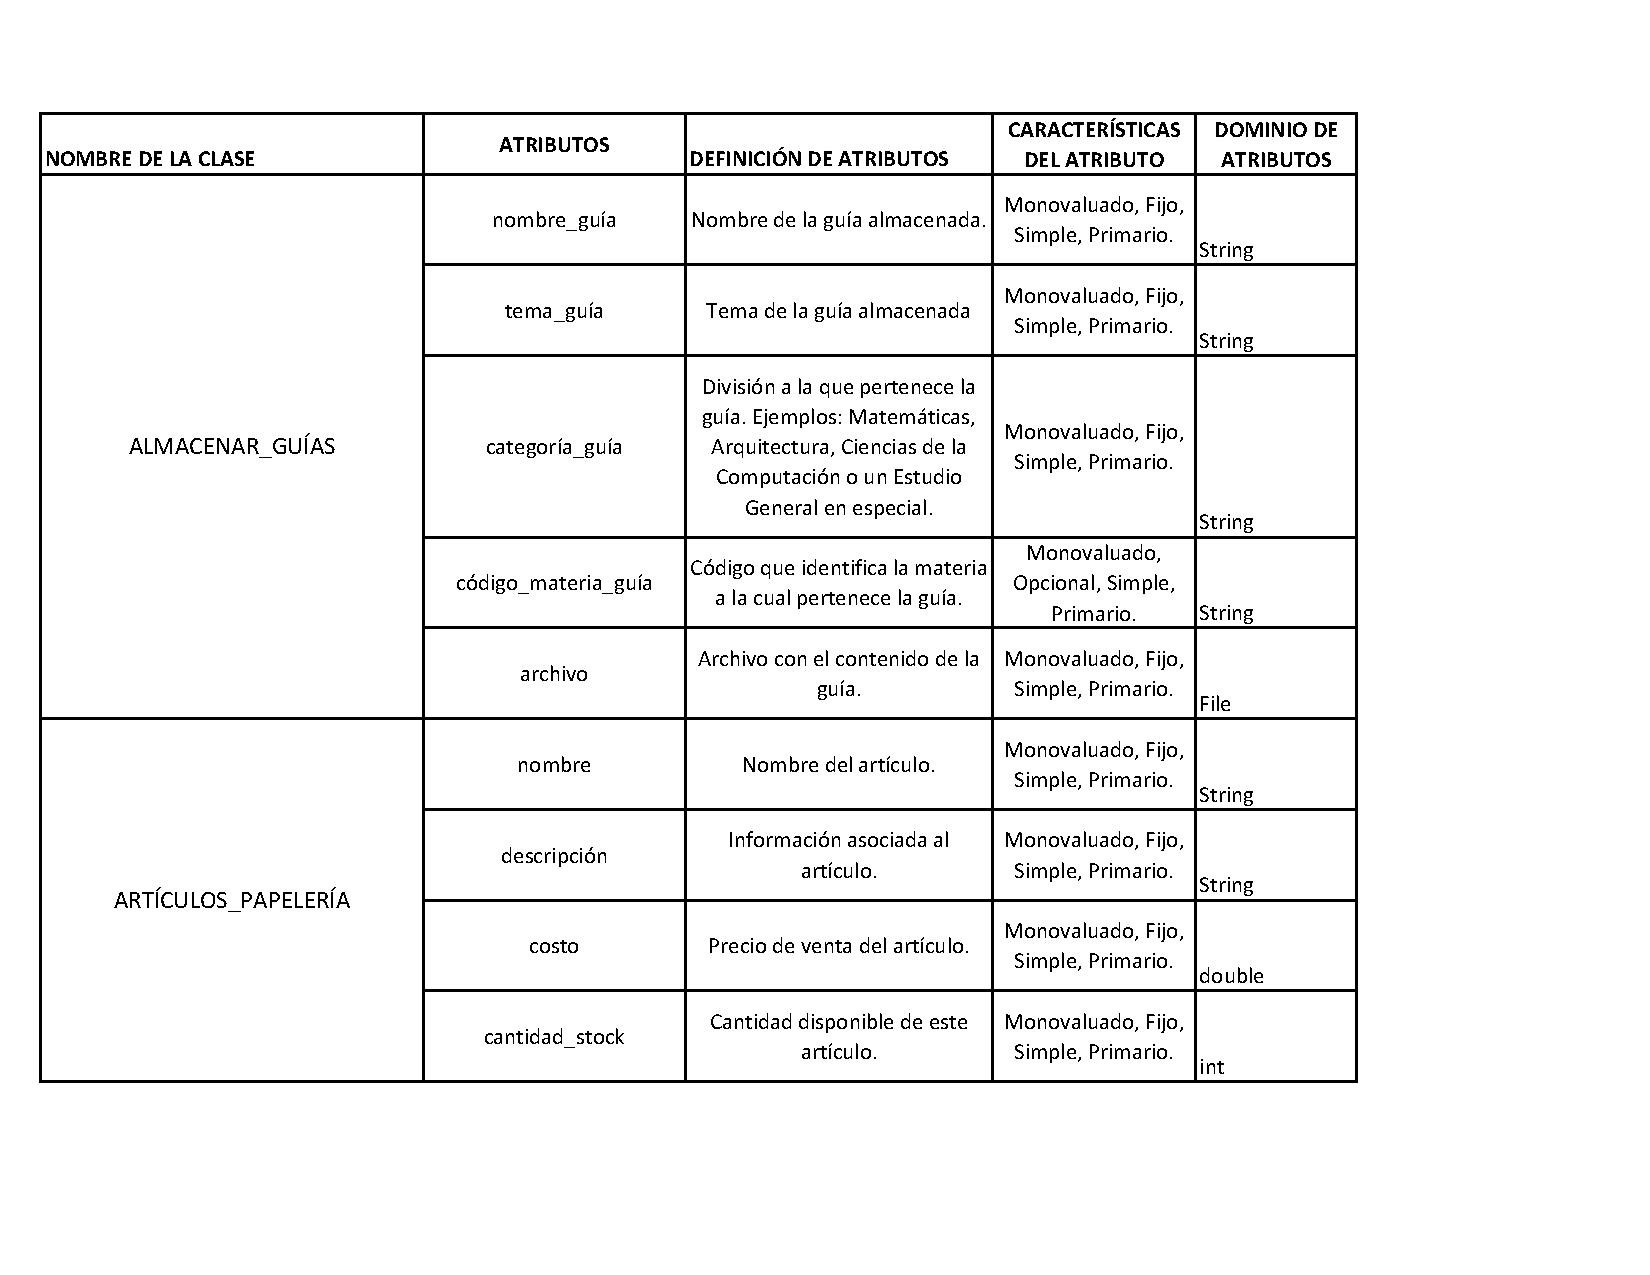
\includepdf[pages=-]{/Users/Julio/Dropbox/CI5311/Proyecto/Fase2/Clasesyatributos.pdf}
\subsection{Descripci\'on de las Clases , Operaciones y
  Restricciones Expl\'icitas}
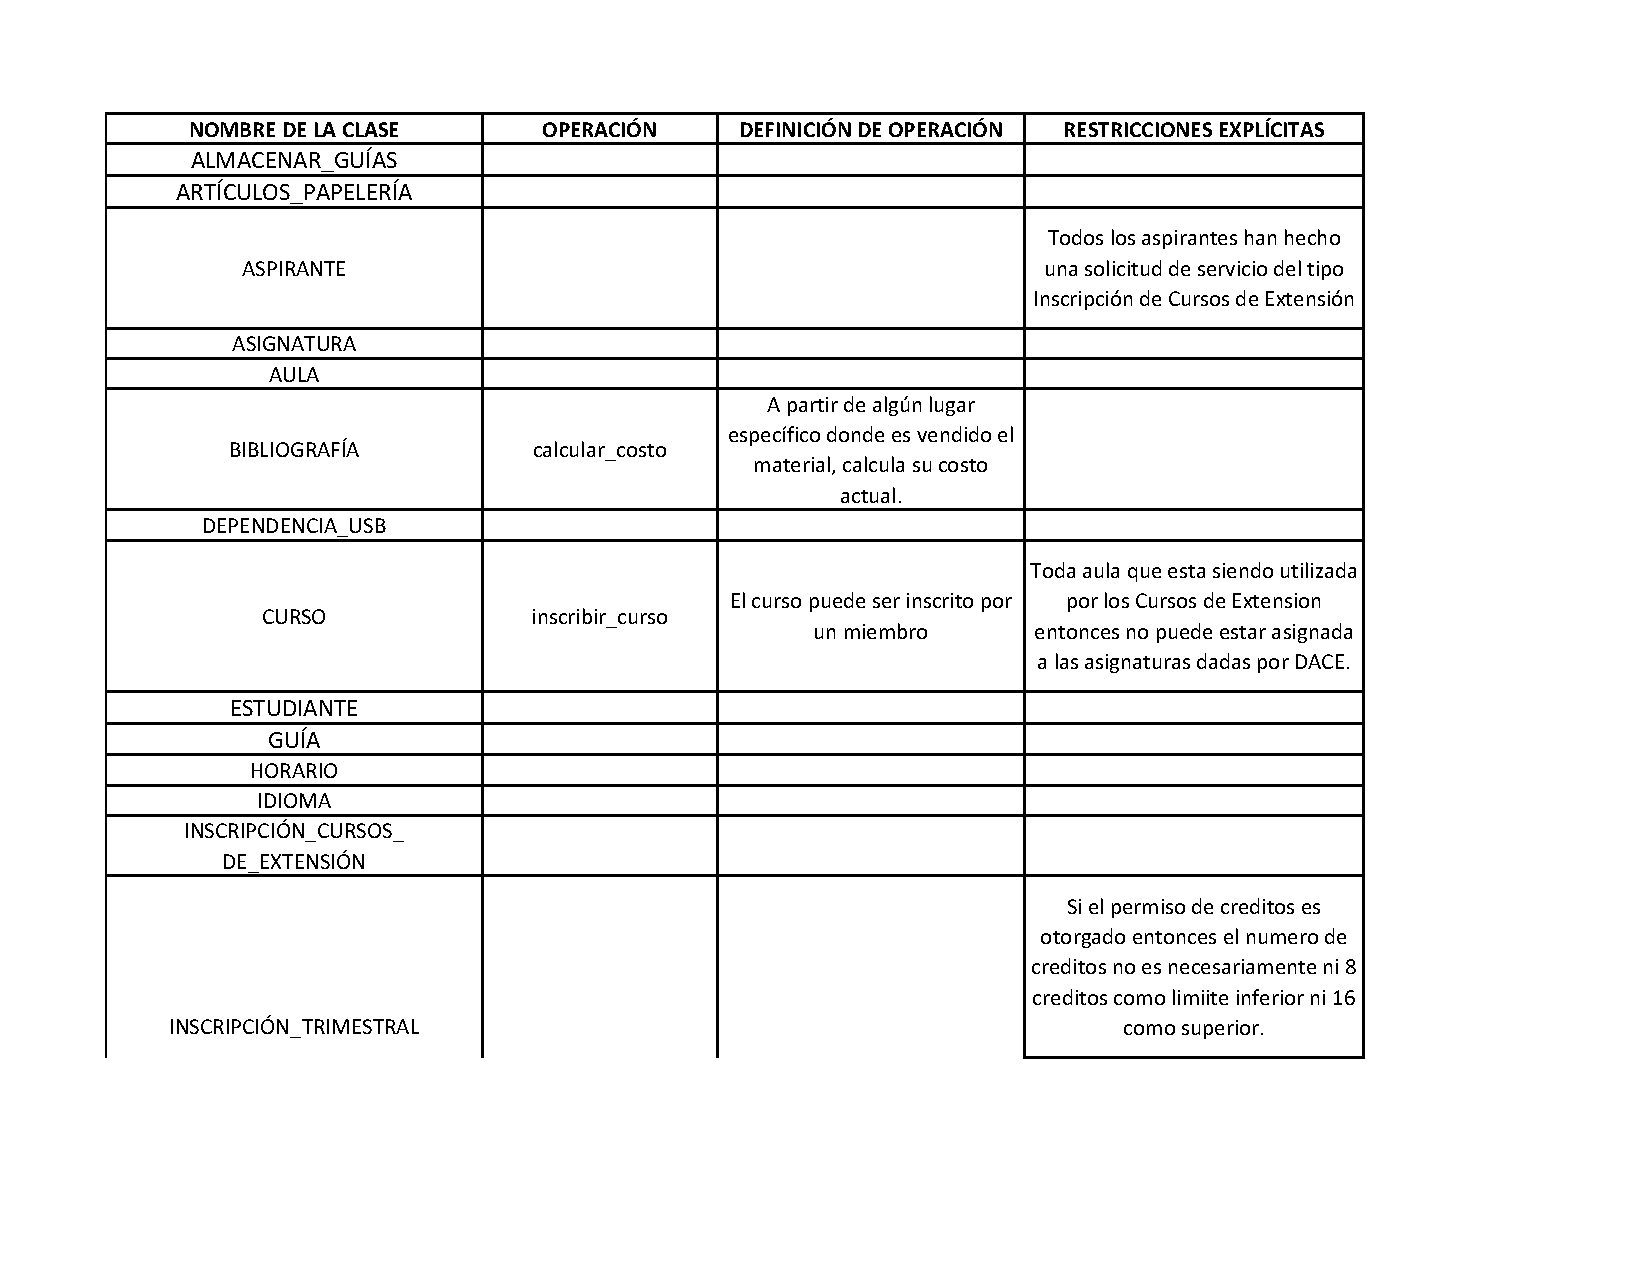
\includepdf[pages=-]{/Users/Julio/Dropbox/CI5311/Proyecto/Fase2/Clasesoperacionesyrestricciones.pdf}
\subsection{Descripci\'on de las Clases, Asociaciones y
  Generalizaciones}
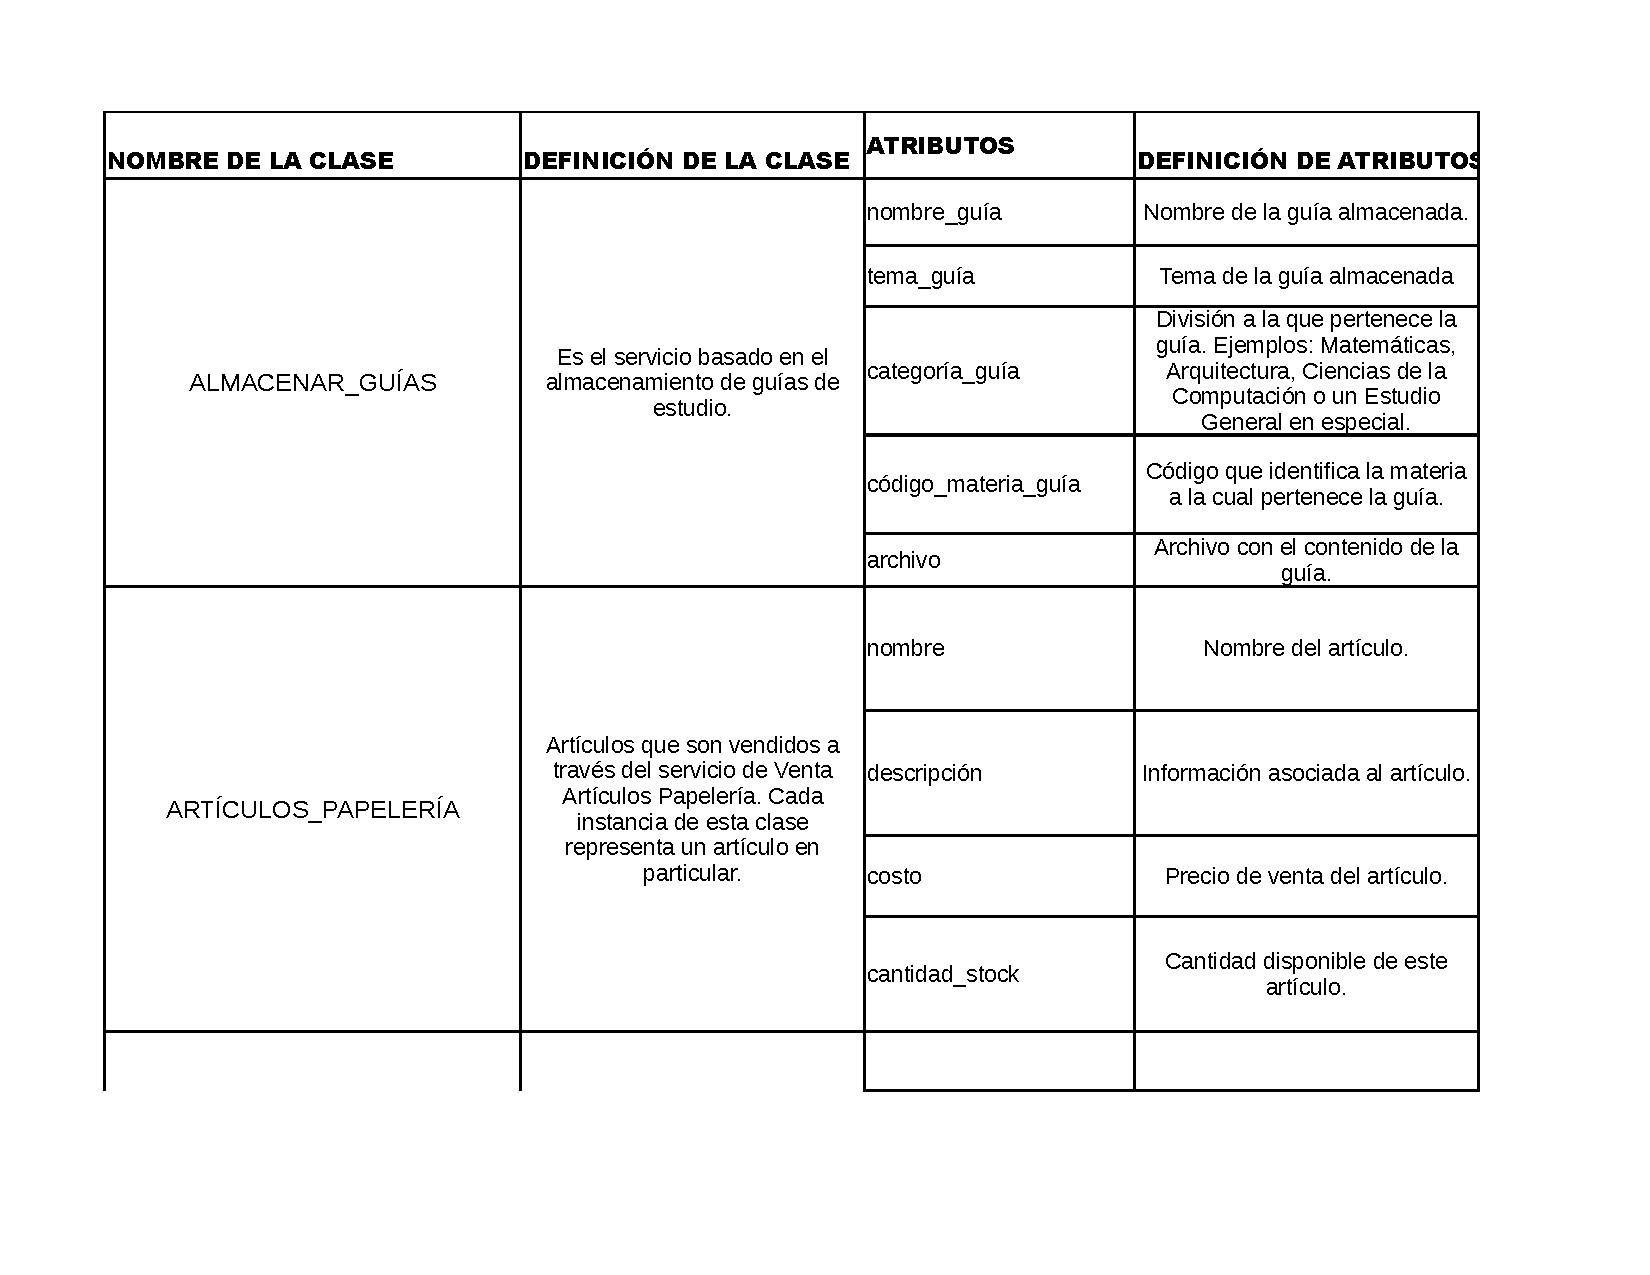
\includepdf[pages=-]{/Users/Julio/Dropbox/CI5311/Proyecto/Fase2/Descripcionclasesasociacionesygeneralizaciones.pdf}

\section{Diagrama del Modelo de Objetos}
\subsection{Visi\'on de la USB}
\begin{landscape}
\begin{figure}
    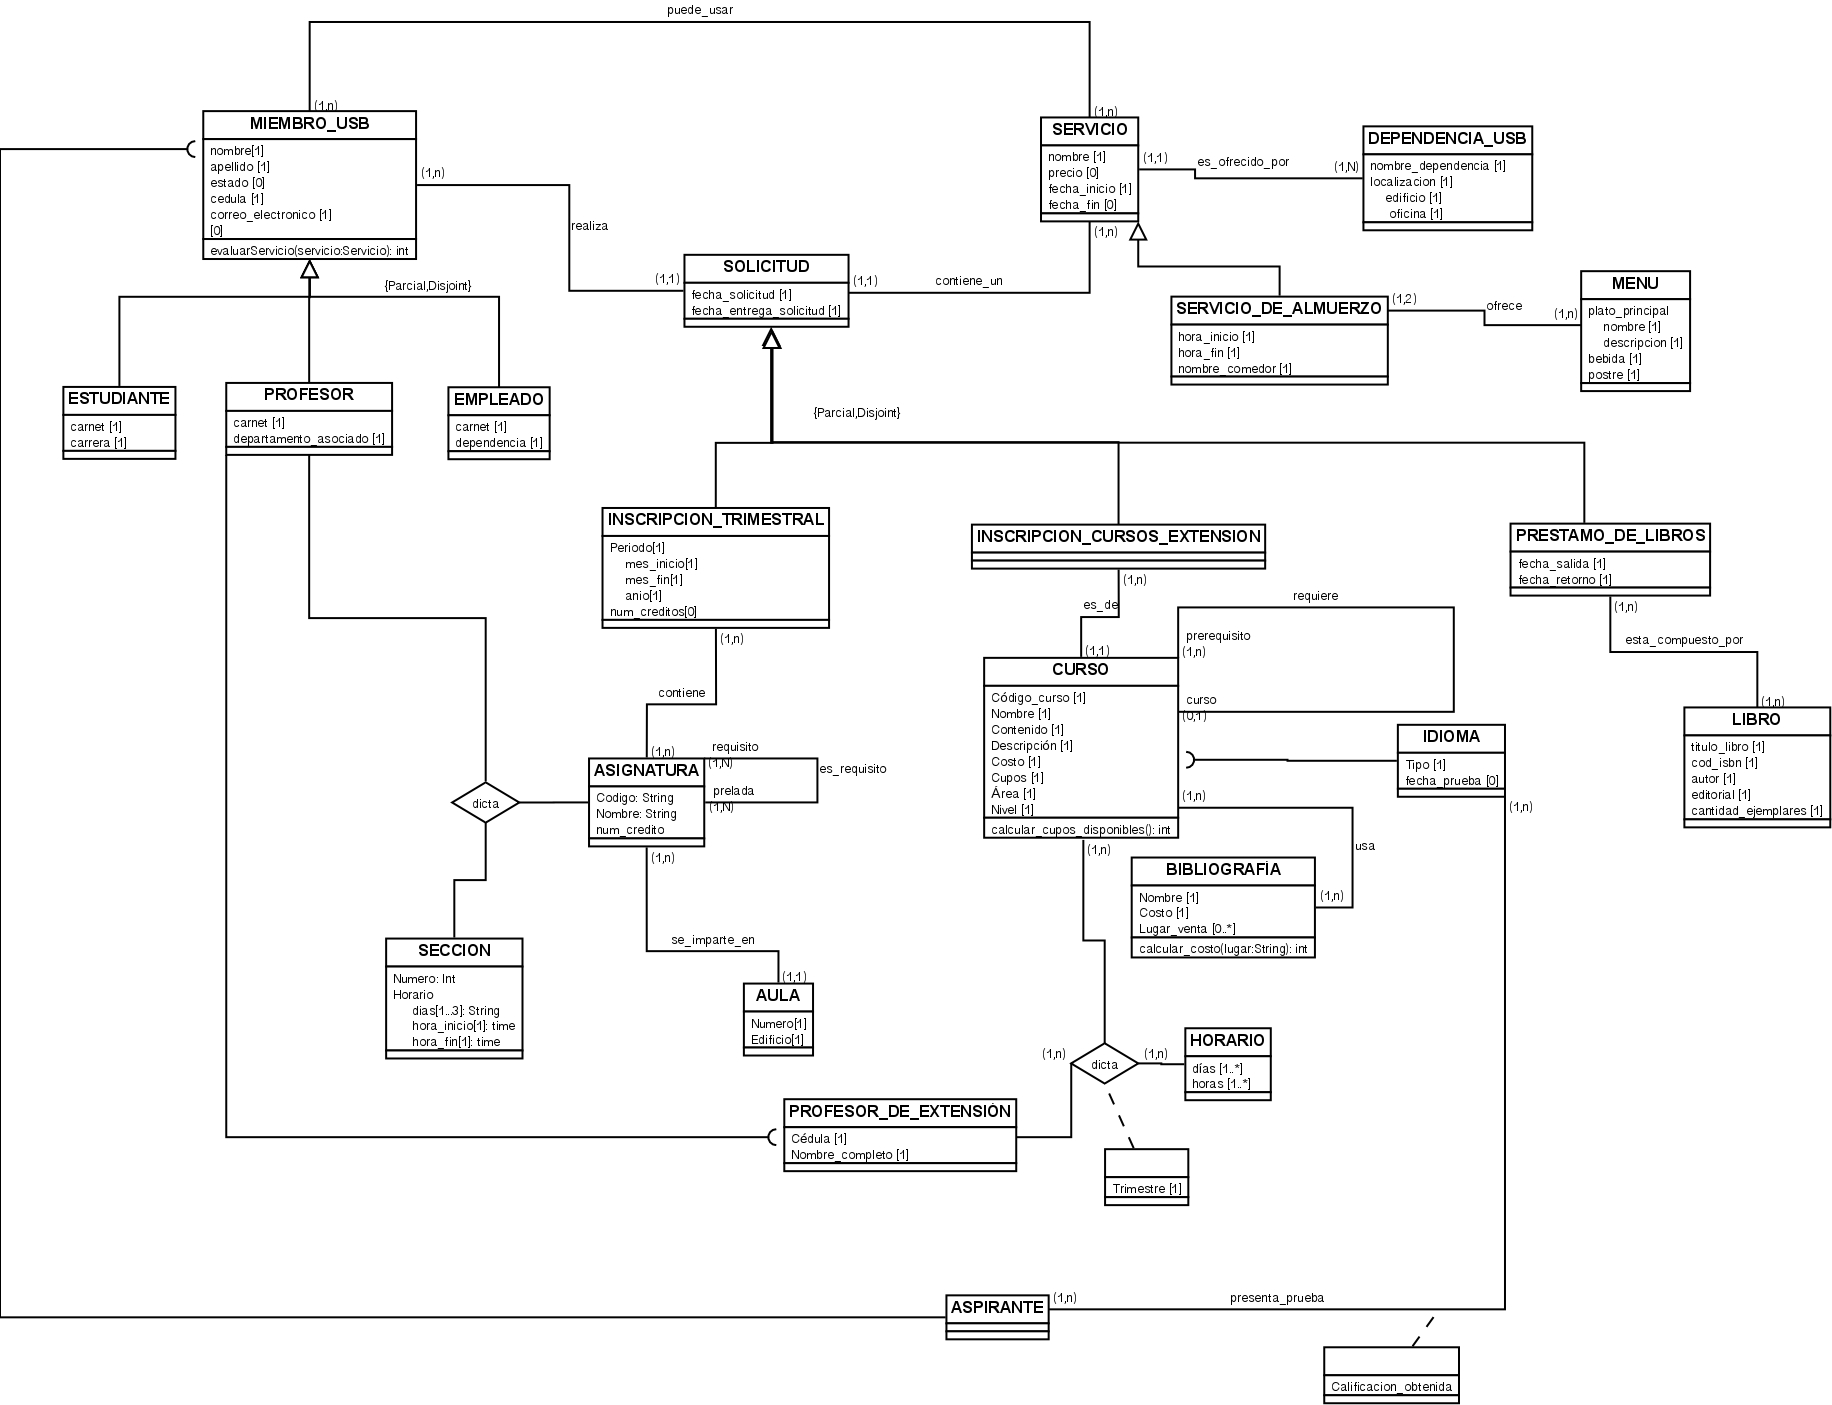
\includegraphics[width=1.59\textwidth]{/Users/julio/Dropbox/CI5311/Proyecto/Fase2/Diagramas/DiagramaUSBNuevo.jpg}
\end{figure} 
\end{landscape}

\newpage
\subsection{Visi\'on de Terceros}
\begin{landscape}
\begin{figure}
    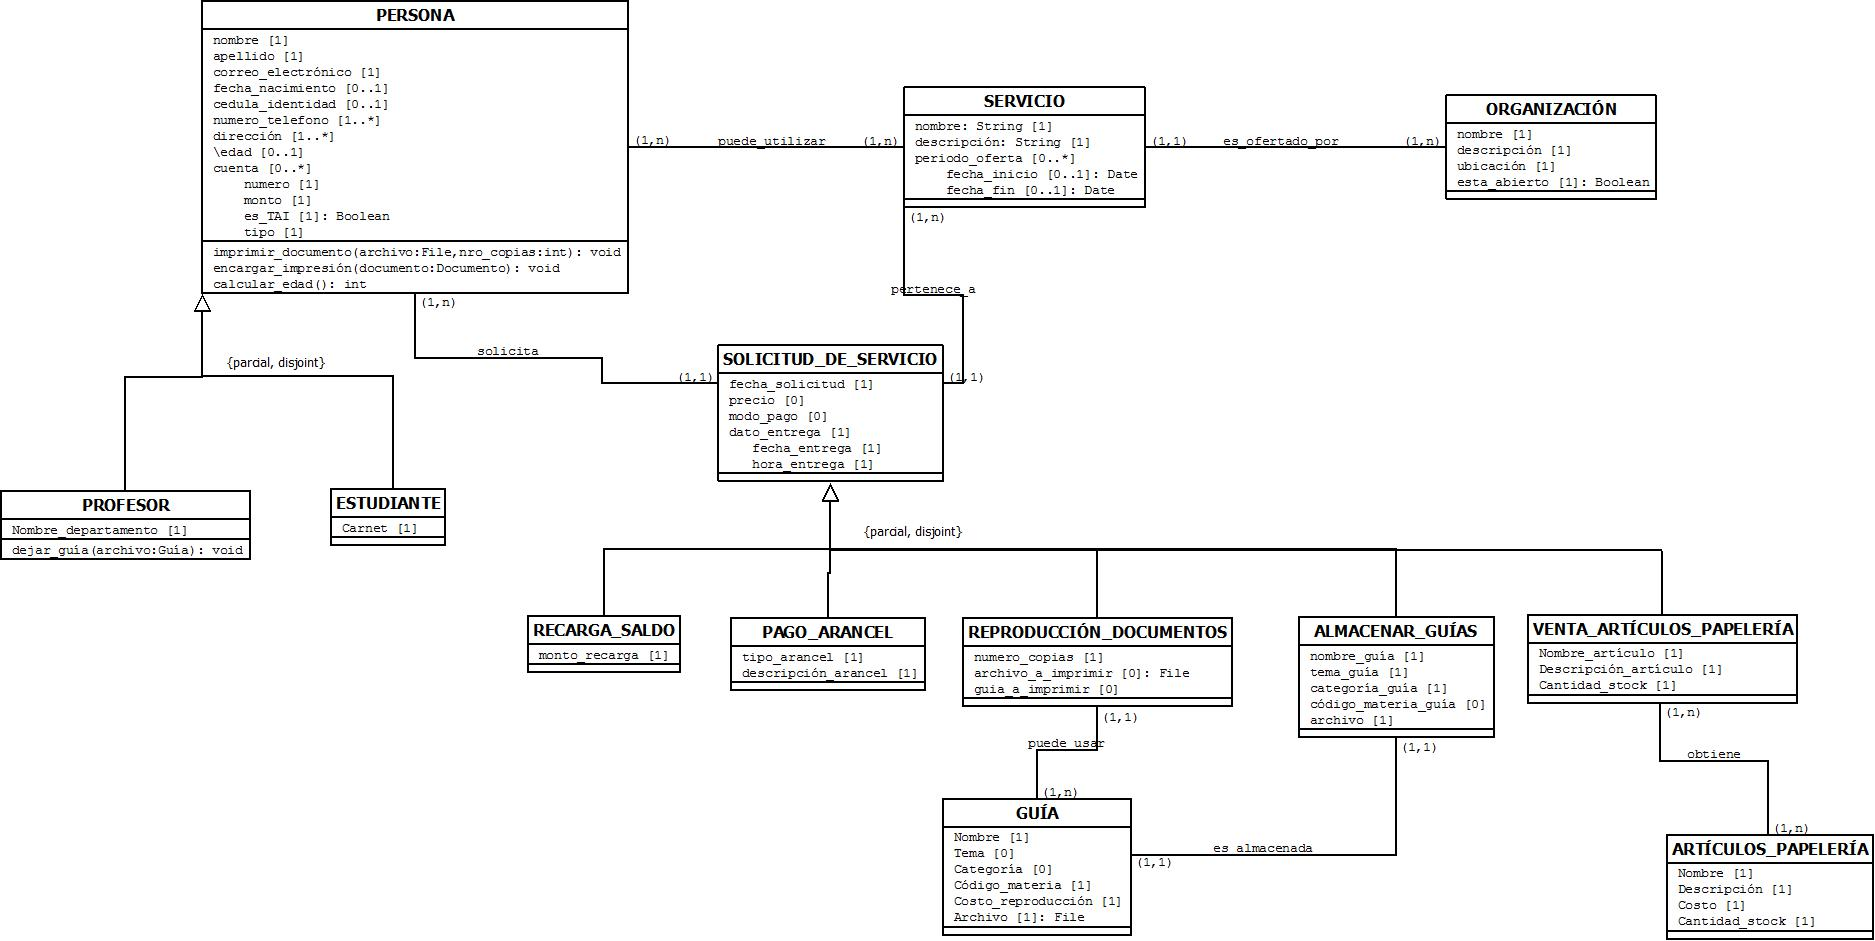
\includegraphics[width=1.83\textwidth]{/Users/julio/Dropbox/CI5311/Proyecto/Fase2/Diagramas/ServicioTerceros.jpeg}
\end{figure} 
\end{landscape}
\newpage

\section{Explicaci\'on de las decisiones de Dise\~no}
 En esta secci\'on se incluir\'an detalles del dise\~no que han podido ser modeladas distinto.
 \newline
 \newline
 
 1. En la clase Miembro USB del diagrama de los Servicios de la USB, se realiz\'o una especializaci\'on en Empleado, Estudiante y Profesor, estos tres tienen en com\'un un carnet,
 el cual pudo haberse modelado como atributo del miembro, sin embargo, este atributo es esencial para poder identificarlos y como la generalizaci\'on es parcial para lograr
 una mayor escalabilidad en el caso de que se quiera agregar otra subclase, entonces se decidi\'o dejarlos especificados en las subclases. De no ser as\'i se hubiese tenido
 que agregar el atributo como opcional y agregar una restricci\'on expl\'icita tal que si el objeto era instancia de alguna de estas tres subclases, el atributo deb\'ia ser distinto
 de nulo.
\newline
\newline

 \subsection{Proceso de Integraci\'on}
 \indent A continuaci\'on se presentar\'an los conflictos encontrados a momento de integrar, se mostrar\'a el an\'alisis, las gu\'ias de modificaci\'on mostrando dos soluciones posibles, finalmente se explicar\'a la soluci\'on seleccionada y la raz\'on por la cual esta opci\'on presentaba m\'as ventaja que las otras. A partir de este momento, para referirnos al Diagrama de Servicios de la Universidad Sim\'on Bol\'ivar ser\'a con \"diagrama USB\" y para el Diagrama de Servicios de Terceros ser\'a como \"diagrama Terceros\" por motivos de facilidad de lectura. 
\subsubsection{Clase Servicio}
\indent En ambos diagramas se presenta un conflicto de estructura con esta clase, ya que en el diagrama USB, la clase Servicio posee los siguientes atributos: Nombre y Precio y en el diagrama Terceros,la clase Servicio adem\'as del atributo \"nombre\", posee como atributos: descripci\'on y periodo de oferta, a su vez compuesto por fecha de inicio y una fecha de finalizaci\'on.
\newline
\newline
\indent Las soluciones planteadas son las siguientes:
\begin{itemize}
\item Mantener la clase Servicio del diagrama de Terceros agregando los atributos no comunes como opcionales.
\item Mantener la clase Servicio del diagrama de Servicios USB agreg\'andole los atributos no comunes de la clase Servicios del diagrama de Terceros como opcionales. 
\end{itemize}
\indent La soluci\'on escogida es la primera debido a que la clase Servicio del Diagrama de Terceros est\'a m\'as completo ya que contempla especificaciones del servicio que permiten una mejor descripci\'on. Al agregar el atributo restante que es Precio como opcional, de ser nulo, no provocar\'ia tanto peso a que si se escogiese la segunda soluci\'on, en el cual la mayor\'ia podr\'ia tener valor nulo.
\subsubsection{Clase Persona y Clase Miembro USB}
\indent La clase Persona del diagrama Terceros y la clase Miembro USB del diagrama USB poseen un conflicto de nombre, son sin\'onimos debido a que tienen la misma sem\'antica, en el sentido en que ambos se refieren a usuarios de servicios ofertados y poseen nombres distintos. Adicionalmente tienen un conflicto estructural ya que aunque como se denot\'o anteriormente poseen la misma sem\'antica, difieren en sus atributos. Tambi\'en estas clases est\'an especializadas cada una por su parte parcialmente con algunas diferencias, esto no presenta un conflicto incompatible, ya que las estas especializaciones comparten la misma sem\'antica.
\newline
\newline
\indent Las soluciones planteadas para el conflicto de nombre son las siguientes:
\begin{itemize}
\item La posible soluci\'on de nombres es poner el mismo nombre en ambas clases. 
\item La primera es colocarle el nombre Persona.
\item La segunda es colocarle el nombre Miembro USB.
\end{itemize}
\indent Las posibles soluciones para el conflicto estructural son:
\begin{itemize}
\item Mantener los atributos de la Clase Persona.
\item Mantener los atributos de la Clase Miembro USB.
\end{itemize}
\indent La opci\'on seleccionada para solucionar el conflicto de nombre es Persona, porque es m\'as general para poder identificar a las personas que hacen vida en la USB y adem\'as a las personas externas.
\newline
\newline
\indent La soluci\'on escogida para el conflicto estructural es mantener los atributos de la Clase Persona, agregando el atributo \emph{estado} de la clase Miembro USB porque Persona tiene atributos como correo electr\'onico, n\'umero telef\'onico que podr\'ian ser datos que le interesar\'ia a Dependencias como DACE para realizar el proceso de inscripci\'on, que aunque no fueron contemplados, le agregan mayor especificidad a los usuarios de los servicios.
\newline
\newline
\indent Se mantiene la clase Empleado de la generalizaci\'on/especializaci\'on de Miembro USB, pero pasa a ser parte de la generalizaci\'on de Persona, debido a que le agrega sem\'antica.
\subsubsection{Clase Solicitud y Solicitud de Servicios}
\indent En las clases Solicitud de Servicios del diagrama de Terceros y Solicitud en diagrama USB tienen conflictos de nombre y estructura. El primero viene dado porque tienen nombres distintos pero la misma sem\'antica, es decir, son sin\'onimos. El segundo viene dado porque a pesar que tienen la misma sem\'antica tienen distintos atributos. 
\newline
\newline
\indent Las soluciones planteadas para el conflicto de nombre son las siguientes:
\begin{itemize}
\item Matener nombre Solicitud
\item Mantener nombre Solicitud de Servicio
\end{itemize}
\indent Las posibles soluciones para el conflicto estructural son:
\begin{itemize}
\item  Conservar la clase Solicitud de Servicios y agregarle los atributos no comunes con respecto a la clase Solicitud.
\item  Conservar la clase Servicio y agregarle los atributos no comunes con respecto a la clase Solicitud de Servicios.
\end{itemize}
\indent Con respecto al nombre, se seleccionar\'a el nombre Solicitud de Servicios ya que es m\'as autoexplicativo. Para la soluci\'on del conflicto estructural, la clase Solicitud de Servicios contiene un conjunto de atributos que ayudan a la expresividad del diagrama.
\subsubsection{Clase Profesor}
\indent En las clases Profesor de ambos diagramas tienen conflicto de estructura, ya que en el Diagrama de USB tiene el carnet y en el otro no. Las posibles soluciones son de nuevo mantenernos con una o la otra, se preferir\'a por motivos de autoexplicaci\'on la clase Profesor en el diagrama USB 
\subsubsection{Clase Estudiante}
\indent En las clases Estudiante de ambos diagramas tienen conflicto de estructura, ya que en el Diagrama de USB tiene el atributo carrera y en el otro no. Al igual que con la clase profesor, tenemos las opciones de quedarnos con una clase o la otra. Se consider\'o que la mejor soluci\'on es mantener la clase Estudiante de USB que contiene mayor informaci\'on.
\subsubsection{Asociaci\'on es\_ofertado\_por}
\indent En ambos diagramas se encuentra esta asociaci\'on que permiten relacionar al Servicio con el ente que lo oferta, pero como el ente en ambos diagramas poseen significados distintos, entonces este conflicto es considerado un hom\'onimo, por lo que, a la asociaci\'on entre Organizaci\'on y Servicio se le cambiar\'a el nombre a es\_dirigido\_por.

\subsection{Diagramas Modificados}
\subsubsection{Visi\'on de la USB}
\begin{landscape}
\begin{figure}
    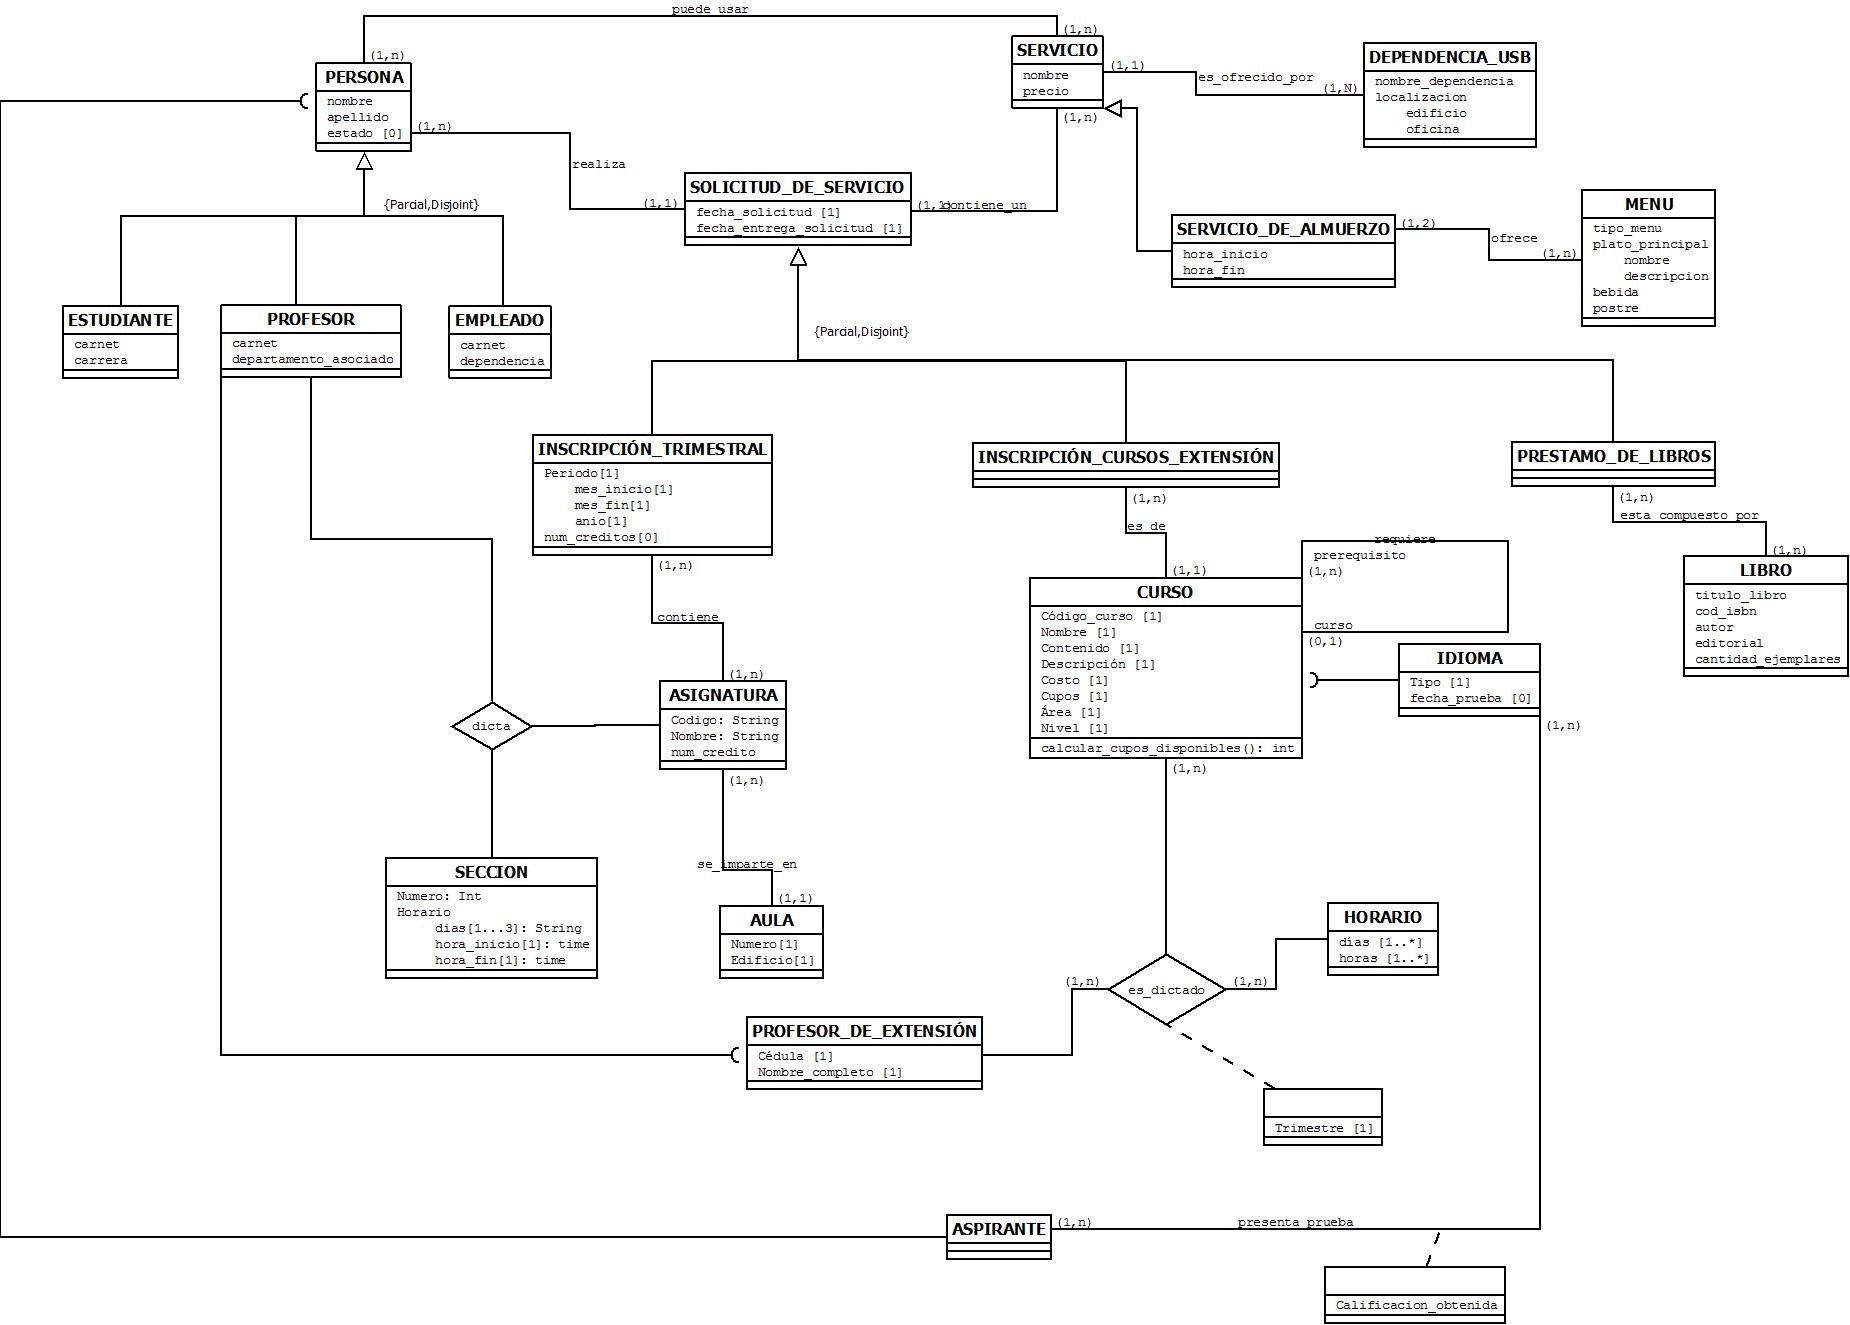
\includegraphics[width=1.7\textwidth]{/Users/julio/Dropbox/CI5311/Proyecto/Fase2/Diagramas/DiagramaUSB_Modificado.jpeg}
\end{figure} 
\end{landscape}
\newpage
\subsubsection{Visi\'on Externa}
\begin{landscape}
\begin{figure}
    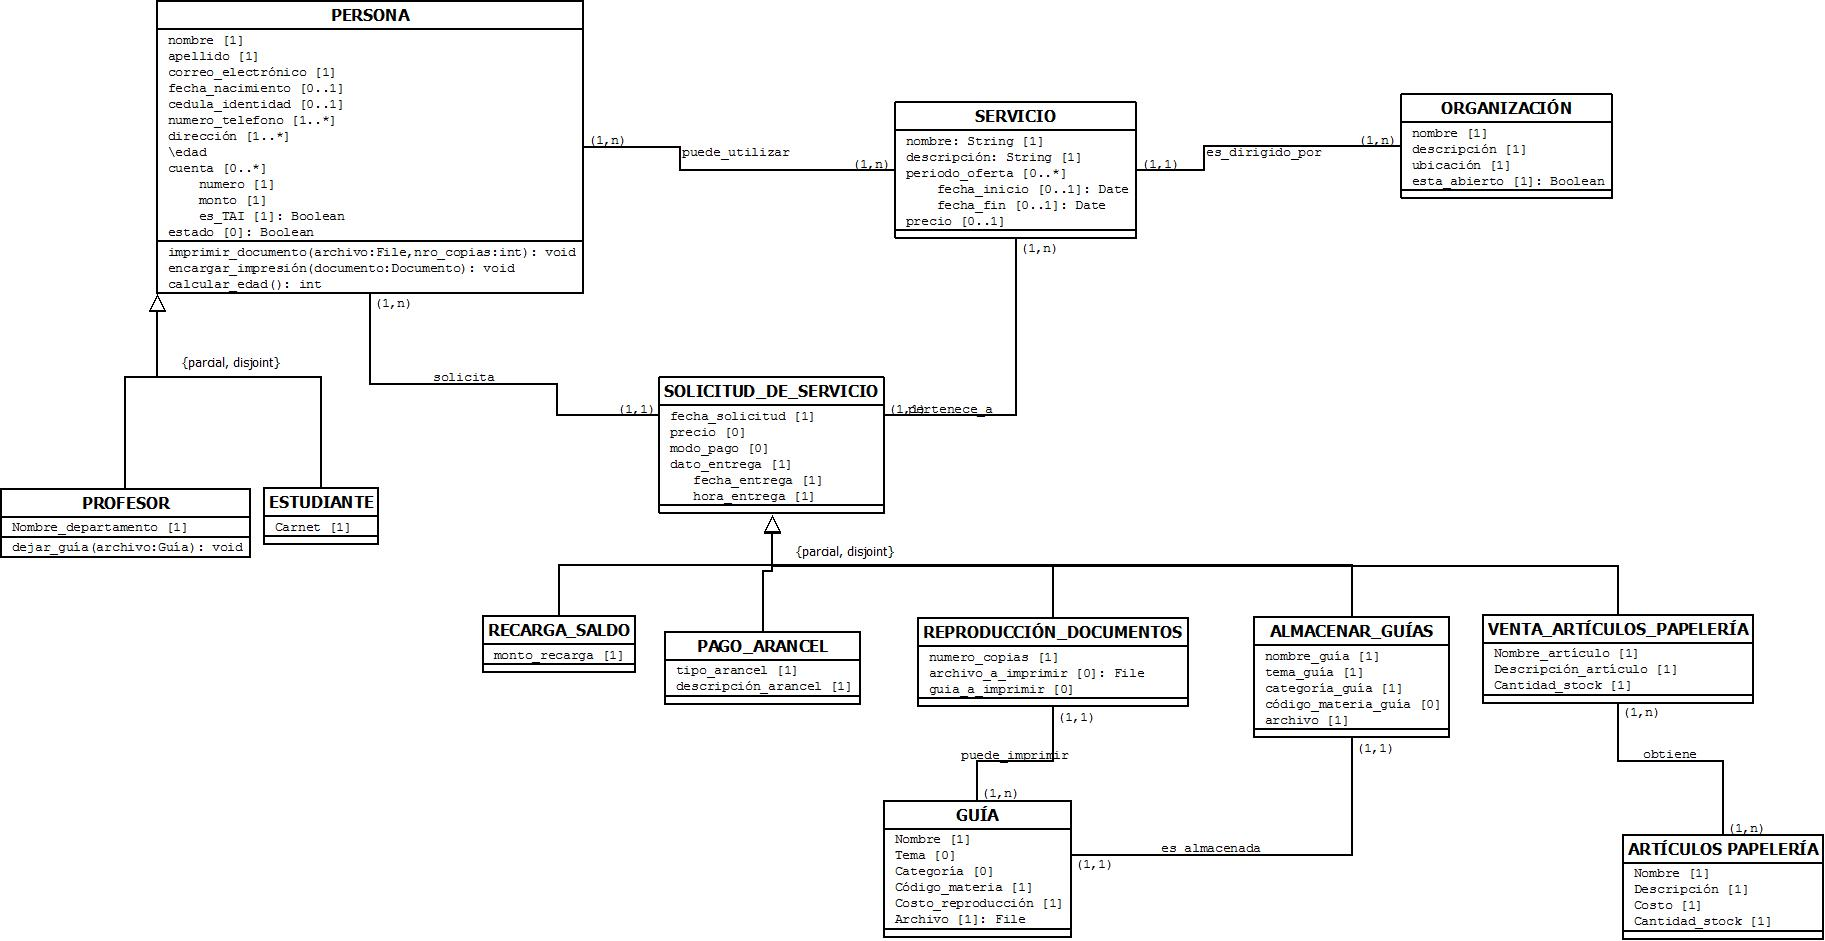
\includegraphics[width=1.8\textwidth]{/Users/julio/Dropbox/CI5311/Proyecto/Fase2/Diagramas/ServicioTercerosModificados.jpeg}
\end{figure} 
\end{landscape}
\subsubsection{Integraci\'on de Vistas}
\begin{landscape}
\begin{figure}
    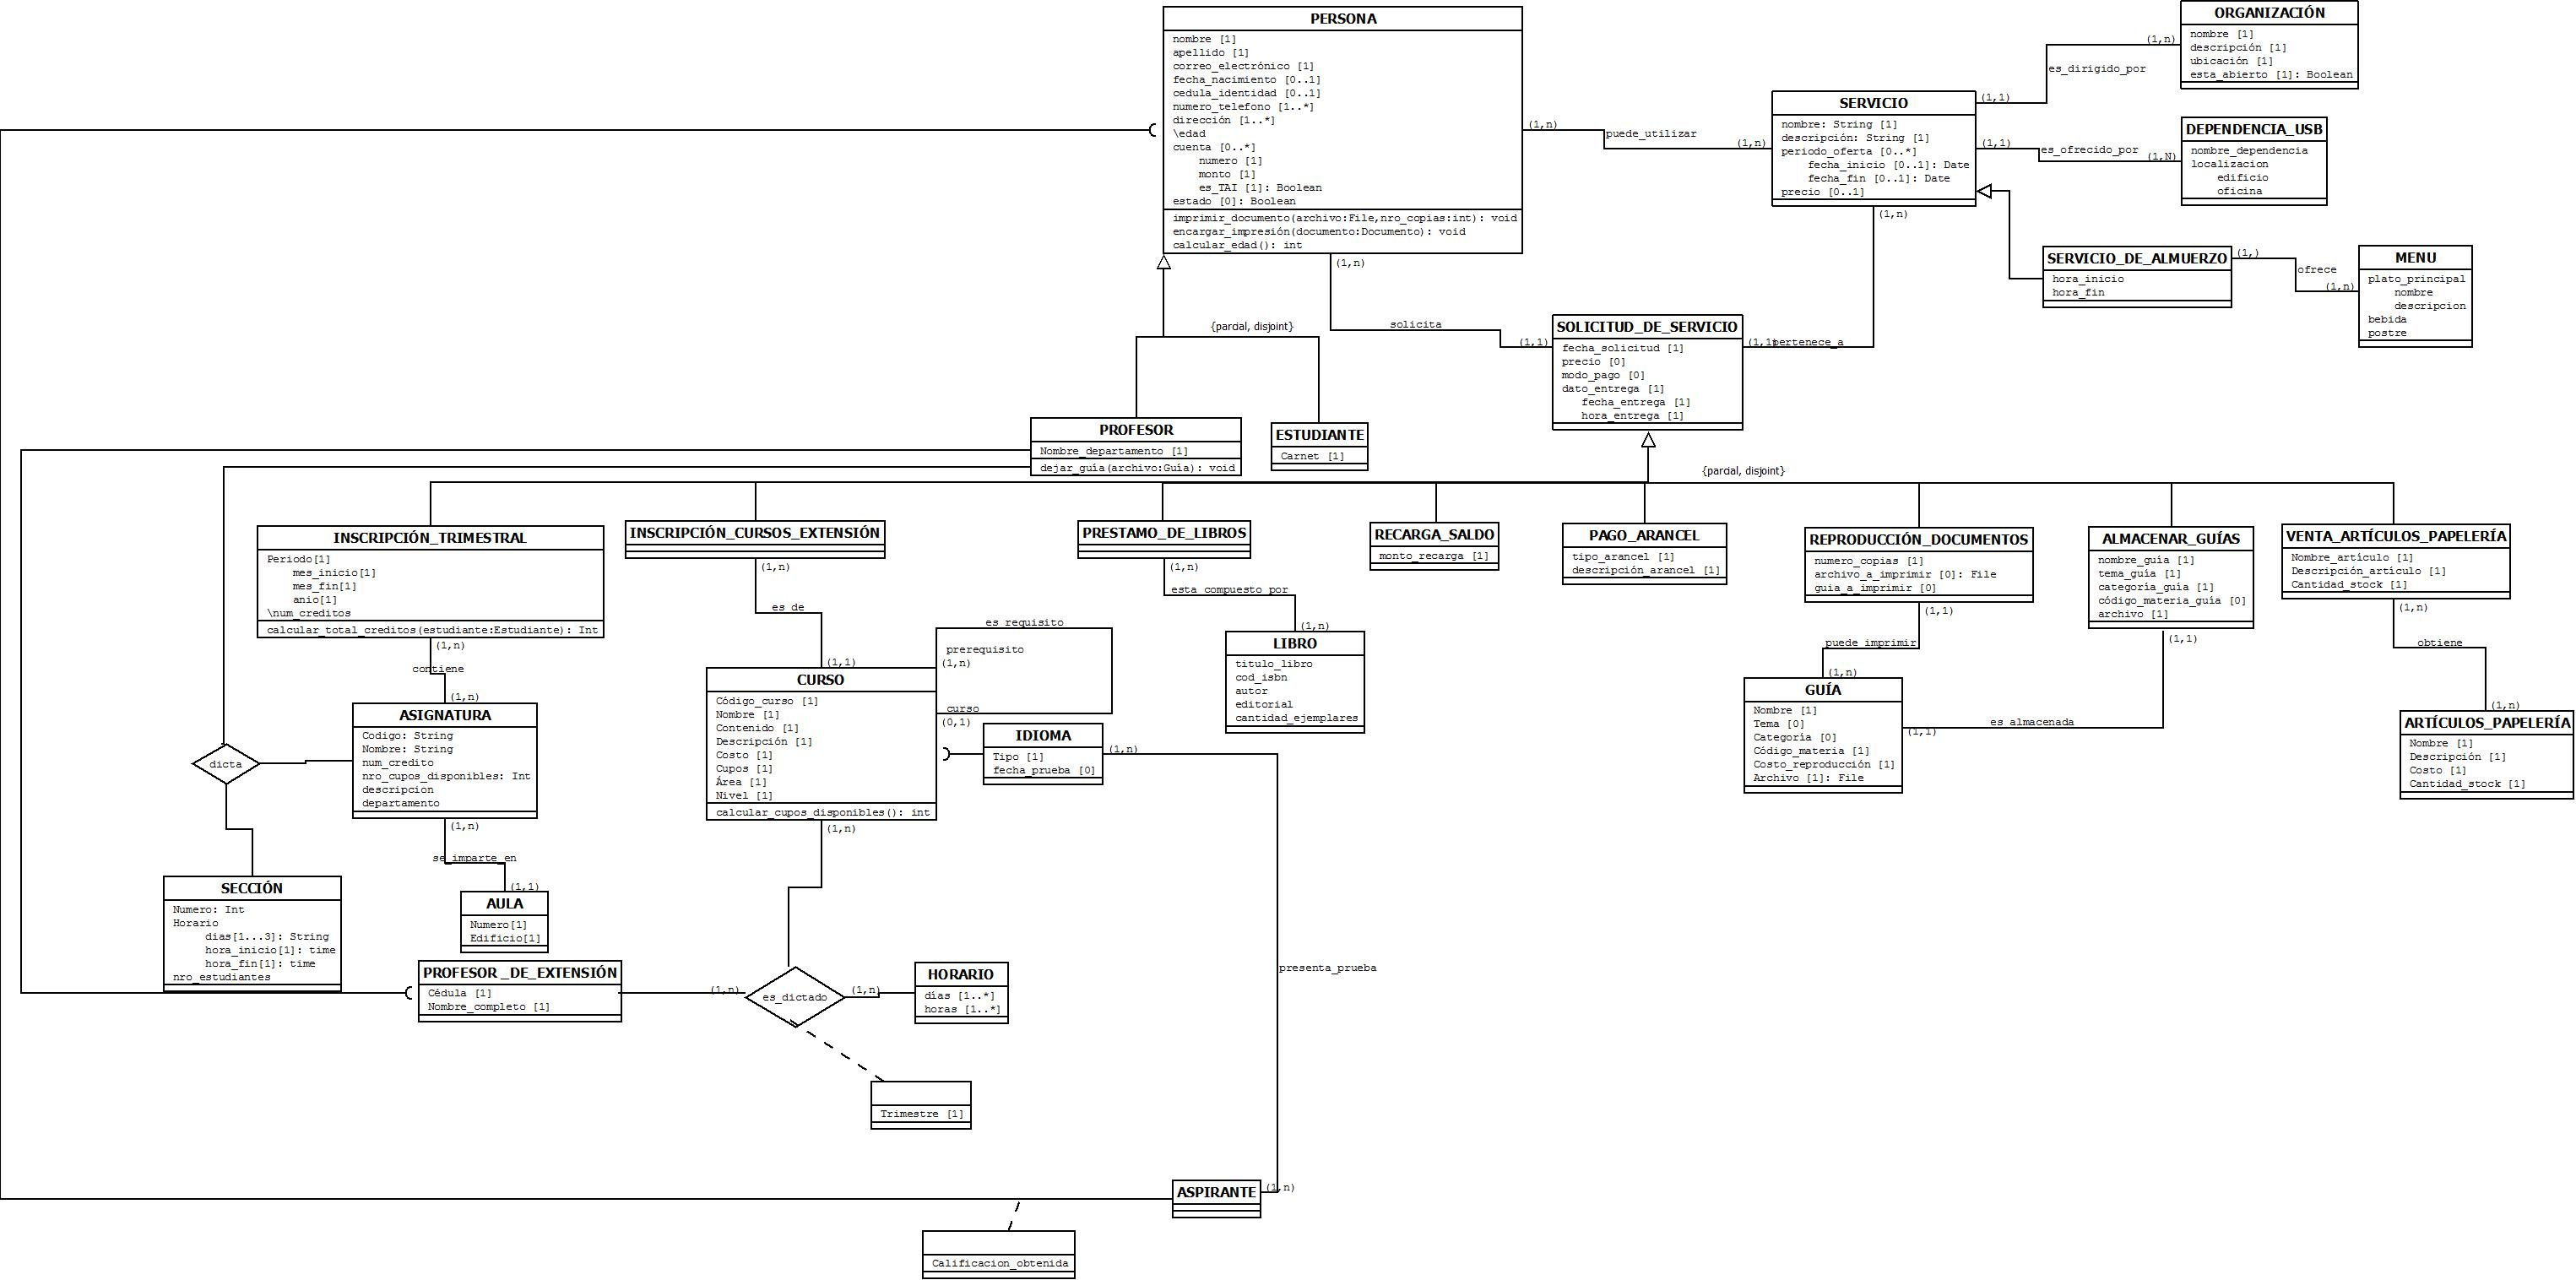
\includegraphics[width=1.85\textwidth]{/Users/julio/Dropbox/CI5311/Proyecto/Fase2/Diagramas/Integrado.jpeg}
\end{figure} 
\end{landscape}
\end{document}